\section{The Privacy Dilemma in Single Sign-On}
\label{sec:challenge}

In this section, we describe the challenges for developing privacy-preserving SSO systems and provide an overview of the solutions proposed in UPRESSO.



\subsection{Basic Security Requirements of SSO}
\label{subsec:basicrequirements}
Both the designs of SSO protocols and the implementations of SSO systems are challenging ~\cite{SPRESSO},
and various vulnerabilities have been found in existing systems~\cite{SomorovskyMSKJ12,WangCW12,ArmandoCCCPS13,ZhouE14,WangZLLYLG15,WangZLG16,YangLLZH16,MainkaMS16,MohsenS16,MainkaMSW17,YangLCZ18,YangLS17,ShiWL19}.
With these vulnerabilities, the adversaries break the security of SSO systems and achieve the following two goals~\cite{SPRESSO}:
\begin{itemize}
\item \textbf{Impersonation}: Adversary logs in to an honest RP as the victim user.
\item  \textbf{Identity injection}: A victim user logs in to an honest RP under the adversaries' identity.
\end{itemize}

We summarize basic requirements of SSO systems based on existing theoretical analysis~\cite{ArmandoCCCT08,FettKS16, FettKS17} and practical attacks~\cite{SomorovskyMSKJ12,WangCW12,ArmandoCCCPS13,ZhouE14,WangZLLYLG15,WangZLG16,YangLLZH16,MainkaMS16,MohsenS16,MainkaMSW17,YangLCZ18,YangLS17,ShiWL19} on SSO systems. These basic requirements focus on  functions and security of SSO systems, and are as follows:

\vspace{1mm}\noindent\textbf{User identification.} When a user logs in to a same RP multiple times, the RP should be able to associate these logins to provide a continuous and personalized service to that user.

\vspace{1mm}\noindent\textbf{Receiver designation.} The receiver designation requires that the identity proof should  be  sent only to the RP (and user) that the user visits, and be bound to this RP so that it will accepted only by this RP.


\vspace{1mm}\noindent\textbf{Integrity and confidentiality.} Only the IdP is able to generate a valid identity proof,
     no other entity should be able to modify or forge it~\cite{WangZLG16} without being found. And, the confidentiality of the identity proof is ensured during the transmission among the IdP, user and the designated RP. While, the correct RP should only accept the valid identity proof.


These basic requirements are the minimum properties that an SSO system has to provide.
User identification is necessary for all services except the anonymous systems which will be discussed in Section~\ref{sec:related},
 therefore RPs should be able to identify the user with the help from IdP.
While either the receiver designation, integrity or confidentiality not satisfied, the impersonation and identity injection will exist in the SSO systems.
For example, without the receiver designation, the adversaries cloud make the victim RP  incorrectly accept the identity proof intended for other RP, which allows the adversary to perform impersonation directly or inject the identity proof in the web session between the victim user and honest RP with other web attacks (e.g., CSRF~\cite{zeller2008cross}); and without integrity, the impersonation and identity injection attacks could be constructed easily  as an adversary could directly modify user's identifier in the identity proof; while without confidentiality, the adversaries cloud use the leaked identity proof to impersonate the victim user at an honest RP~\cite{ChenPCTKT14,FettKS16,WangZLG16}.



\subsection{The Privacy Dilemma and Existing Attempts}
\label{subsec:challenges}
In addition to the basic requirements, a privacy-preserving SSO system should prevent the IdP-based access tracing %login tracing 和 access tracing 没有已经广泛使用的说法
and RP-based identity linkage.
In details, the privacy-preserving SSO system should prevent the curious IdP from obtaining any information that could identify the user's accessed RP (for example, through RP's identifier and URL) or associate the logins at an RP,
and prevent  the collusive RPs from associating a user's logins at different RPs.

The privacy-preserving requirements need to be integrated into the basic requirements, to protect the user privacy under the prerequisite that the correct functions and security of SSO systems are ensured.
The privacy-preserving user identification requires IdP to provide a user's identifier ($PID_U$) to help the RP in identifying the user locally,
 under the prerequisites that the curious IdP can never identify the visiting RP or classify logins based on RP and the collusive RPs cannot find the correlation between $PID_U$s for a user.
The privacy-preserving receiver designation requires IdP (or the user) to bind an identity proof with an RP and send it only to this RP,
 while IdP can never identify the RP visited by the user or classify logins based on RP.

\begin{figure}
  \centering
  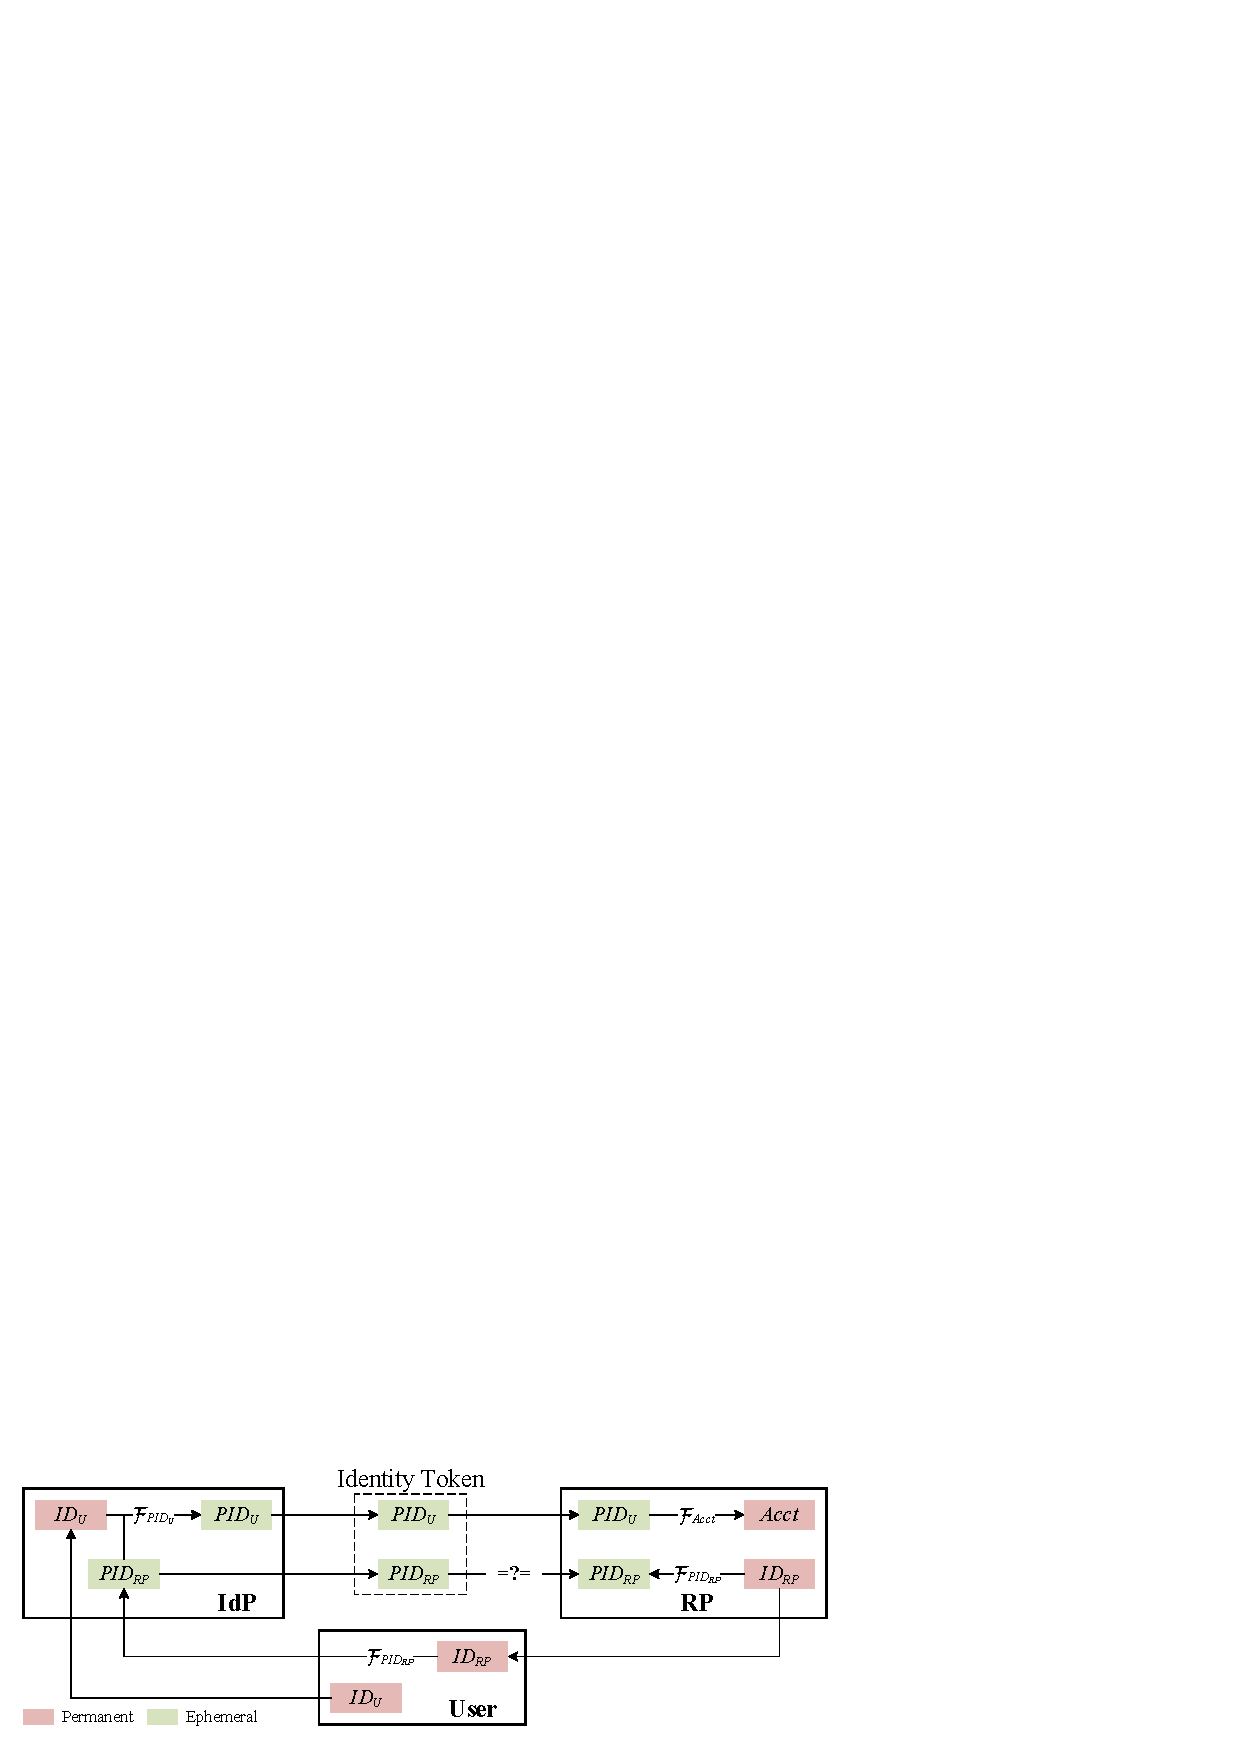
\includegraphics[width=\linewidth]{fig/IDCorrelation.pdf}
  \caption{ID transformations in a privacy-preserving SSO system.}
  \label{fig:IDCorrelation}
\end{figure}

The above analysis demonstrates that the identifers of the user and RP need to be carefully processed in SSO systems.
Here, we systematically analyze the forms of the user and RP identifiers, as required by privacy protection.
As in Figure~\ref{fig:IDCorrelation},
 IdP, who knows the user's globally unique identifer ($ID_U$), should only obtain a privacy-preserving identifer for an RP ($PID_{RP}$);
 each RP, who knows its globally unique identifer ($ID_{RP}$), should only receive a privacy-preserving identifer for a user ($PID_{U}$) from the identity proof.
The $PID_{RP}$ may be null, it means IdP has no information about RP, for example in BrowserID~\cite{BrowserID}.
The $PID_{U}$ can never be null, as RP has to derive the $Accout$ from it, which is the basic function of SSO systems.
Here the  privacy-preserving identifers in multiple sessions will never leak the globally unique identifer nor link the sessions from an entity (the RP and user).
That is, $PID_{RP}$s in multiple sessions for a same RP  should be independent from the view of the IdP;
 and for the collusive RPs, their obtained $PID_{U}$s for a same user should be independent.

Then, we analyze the generation and use of $PID_U$ and $PID_{RP}$, considering the basic requirements of SSO system.
\begin{itemize}
  \item %Who generates $PID_U$? 必须由IdP负责生成PID_U
        IdP is the only trusted entity to control the generation of $PID_U$, as the user is not trusted by the RP and a malicious user may provide incorrect $PID_U$. Here, the ``control" means, IdP may generate $PID_U$ alone or with the corporation from the user, but it's the IdP who finally determines the value of $PID_U$. For clarity, we assume IdP generates $PID_U$ by invoking $\mathcal{F}_{ID_{U} \mapsto PID_{U}}$ with $ID_U$ and $PID_{RP}$, without loss of generality.

  \item %What's the requirement considering $PID_{U}$ and $PID_{RP}$ together? $PID_{U}$ and $PID_{RP}$一起考虑时需要满足的。
  The generation of $PID_{U}$ and $PID_{RP}$ must ensure the \textbf{user identification},
  that is, the RP could derive a same $Account$ with the $PID_{U}$ and $PID_{RP}$ from different logins. We assume RP calculates $Account$ by invoking $\mathcal{F}_{PID_{U} \mapsto Account}$ with $PID_U$, $ID_{RP}$ and $PID_{RP}$.

  \item %Who generates $PID_{RP}$, and what's the requirement? PID_RP可以由RP或者user合作生成,但要保证唯一性。
  Each $PID_{RP}$ must be globally unique, i.e., only assigned to one RP,  for achieving the \textbf{receiver designation}.
        The user and RP may generate the $PID_{RP}$ separately or cooperatively, through the function $\mathcal{F}_{ID_{RP} \mapsto PID_{RP}}$.
        However, both the user and RP must check the uniqueness of $PID_{RP}$ before accept and use it.
        If either the user or the RP doesn't perform the check, the adversary could make it accept a $PID_{RP}$ same as an RP and then misuse the identity proof.
        %$PID_{RP}$ is one form of the RP's identifer, and seems unrelated with the user's identifier.
        %Although, the user may inject the user's information into $PID_{RP}$, these information will be treated as random values at the RP and never be used to calculate $Account$, as the user is not trusted by the RP.
        %Therefore, we can assume that $PID_{RP}$ is generated through $\mathcal{F}_{ID_{RP} \mapsto PID_{RP}}$ with the parameter $ID_{RP}$.~\footnote{The $PID_{RP}$ may also be related with the previous $PID_{RP}$. We omit the previous $PID_{RP}$ in the parameters as it is also a transformation of $ID_{RP}$.}
  \item The \textbf{receiver designation} further requires that  $PID_{U}$ is bound with either a non-null $PID_{RP}$ or $ID_{RP}$ in identity proof.
        When $PID_{RP}$  is non-null, IdP builds the identity proof separately and the \textbf{integrity} is also ensured.
        When $PID_{RP}$  is null, only the user cloud bind $PID_{U}$ with an RP identifier (i.e., $ID_{RP}$) which is unique and checkable to the RP.
        In this case, the user who performs the binding, must have a publicly verifiable grant from the IdP, as required by \textbf{integrity}.
        The binding and integrity cloud be achieved by existing public key infrastructure.
   \item The \textbf{receiver designation} also requires the identity proof will only be sent to the correct RP.
       As IdP doesn't know $ID_{RP}$, the user or a third party trusted by the correct RP will ensure this.
\end{itemize}

Then, the dilemma in the design of a secure and privacy-preserving SSO system, could be transformed into finding three  privacy-preserving ID transformation functions  $\mathcal{F}_{ID_{RP} \mapsto PID_{RP}}$, $\mathcal{F}_{ID_{U} \mapsto PID_{U}}$,  and $\mathcal{F}_{PID_{U} \mapsto Account}$, which satisfying:
\begin{itemize}
  \item For an RP, $\mathcal{F}_{ID_{RP} \mapsto PID_{RP}}$ generates $PID_{RP}$s in multiple logins, and these  $PID_{RP}$s are independent to the IdP.
  \item For a user, $\mathcal{F}_{ID_{U} \mapsto PID_{U}}$ generates $PID_{U}$s in multiple logins at different RPs, and these $PID_{U}$s are independent to these RPs. $\mathcal{F}_{PID_{U} \mapsto Account}$ outputs $Account$s for a user at different RPs, and these $Account$ are independent to these RPs.
  \item For a user and an RP, $\mathcal{F}_{PID_{U} \mapsto Account}$ generates a unchanged $Account$ in multiple logins.
\end{itemize}

Various solutions~\cite{OpenIDConnect, SAMLIdentifier,BrowserID,SPRESSO}, are proposed, attempting to construct a secure and privacy-preserving SSO system.
However, these scheme provide at most two satisfying functions, and therefore fail to prevent either the IdP-based access tracing or RP-based identity linkage.
\begin{itemize}
  \item The traditional SSO systems provide no satisfying functions, and therefore fail to protect the user's privacy.
  \item SAML~\cite{SAMLIdentifier} and OIDC~\cite{OpenIDConnect} provide only the satisfying $\mathcal{F}_{ID_{U} \mapsto PID_{U}}$ and $\mathcal{F}_{PID_{U} \mapsto Account}$ .
        The IdP obtains the $ID_{RP}$ for an RP, and generates the unchanged $PID_{U}$ for the same couple $<ID_{U}$, $ID_{RP}>$,
        while the $PID_{U}$ are independent for different $ID_{RP}$s.
  \item BrowserID~\cite{BrowserID} and SPRESSO~\cite{SPRESSO} provide only the satisfying $\mathcal{F}_{ID_{RP} \mapsto PID_{RP}}$.
        In BrowserID, IdP obtains a null $PID_{RP}$ and provides $ID_U$ to the RP, therefore each RP obtains the unchanged $Accout$.
        In SPRESSO, each RP generates $PID_{RP}$ by encrypting $ID_{RP}$ padding by a random nonce,
        and IdP provides the unchanged $ID_U$ for a user's multiple logins no matter which RP the user is visiting.
\end{itemize}

Obliviously, existing attempts fail to provide the complete  privacy.
The essential reason is that these schemes provide an unchanged value (e.g., $PID_{U}$ in SAML~\cite{SAMLIdentifier} and OIDC~\cite{OpenIDConnect}, or $ID_U$ in BrowserID~\cite{BrowserID} and SPRESSO~\cite{SPRESSO}) for the user's multiple logins at an RP.
To provide unchanged $PID_{U}$, IdP has to know $ID_{RP}$ and then will be able to identity or link the logins at an RP.
Providing $ID_U$ to the RP, makes  the collusive RPs easily link the user's logins at different RPs.


\subsection{The Principles of UPRESSO}
\label{subsec:solutions}
In this work, we present UPRESSO, a secure and privacy-preserving SSO system,
which prevents the IdP-based access tracing and RP-based identity linkage under the prerequisites that  the basic requirements of SSO systems are satisfied.
UPRESSO adopts the public key infrastructure to ensure the integrity of the identity proof and TLS for its confidentiality, which is the same as other SSO systems.
Therefore, we focus on how to provide the privacy-preserving user identification and receiver designation as follows:

\vspace{1mm}\noindent \textbf{Trapdoor user identification.} UPRESSO breaks the implicit assumption in previous SSO systems, that an RP should obtain an unchanged value to identify a user in the multiple logins.
A trapdoor identification is introduced, which allows the RP  to derive the unchanged $Accout$ from different $PID_{U}$s.
The trapdoor identification requires a cooperation of the three functions $\mathcal{F}_{ID_{RP} \mapsto PID_{RP}}$, $\mathcal{F}_{ID_{U} \mapsto PID_{U}}$ and $\mathcal{F}_{PID_{U} \mapsto Account}$.
$\mathcal{F}_{ID_{RP} \mapsto PID_{RP}}$  is invoked with a trapdoor to generate $PID_{RP}s$ which are independent to IdP (preventing IdP-based access tracing),
 and RP uses $\mathcal{F}_{PID_{U} \mapsto Account}$ with this trapdoor to derive the unchanged $Accout$  from $PID_{U}$s that are generated by IdP with $\mathcal{F}_{ID_{U} \mapsto PID_{U}}$.

\vspace{1mm}\noindent \textbf{Transformed receiver designation.}
UPRESSO splits the receiver designation into two steps: IdP designates the identity proof to a transformed RP identifer (i.e., $PID_{RP}$), and the user designates the $PID_{RP}$ to the correct $ID_{RP}$.
 Each RP checks the  designation of the identity proof based on $PID_{RP}$.
And, the designation between $PID_{RP}$ and $ID_{RP}$ ensures that $PID_{RP}$ is correct and the identity proof is only sent to the correct RP.
In the challenging first step, the IdP generates $PID_U$ for $PID_{RP}$ and achieves full privacy-preserving binding (i.e., $PID_U$ with $PID_{RP}$).
UPRESSO introduces an efficient one-way (trapdoor) function $\mathcal{F}_{ID_{U} \mapsto PID_{U}}$.
 It allows IdP to  compute $PID_U$ easily,  avoiding the generation of $PID_U$ to be the bottleneck at a high-throughput IdP;
   and also prevents the RP from finding any information about $ID_U$, which is required by preventing RP-based identity linkage.
As IdP only knows $PID_{RP}$ and has no other information about RP, the user is required to perform the necessary checks  in the second step.
The user will check that $PID_{RP}$ is global unique and corresponding to the correct RP.
Finally, the user sends the identity proof  to the only correct RP.

To meet the above two principles, we need to construct three satisfying functions $\mathcal{F}_{ID_{RP} \mapsto PID_{RP}}$, $\mathcal{F}_{ID_{U} \mapsto PID_{U}}$ and $\mathcal{F}_{PID_{U} \mapsto Account}$, design the protocols between the user, RP and IdP to avoid the privacy leakage during message transmission, and implement the  processing at the user as  required by the transformed receiver designation.









